\section{Parametrized Neural Network}
\subsection{Discriminating Masses}
In figure \ref{fig:PNN50250Dist} I have drawn the distribution of the output from the trained \ac{PNN} architecture 
(see section \ref{subsec:PNNArch}). The model was trained using the FS-MLM data set. In figure \ref{fig:PNN50250Dist},
4 signals have been included; ($\tilde{\chi}_1=50$, $\tilde{\chi}_2=250$GeV), ($\tilde{\chi}_1=100$, $\tilde{\chi}_2=200$GeV), 
($\tilde{\chi}_1=200$, $\tilde{\chi}_2=300$GeV) and ($\tilde{\chi}_1=150$, $\tilde{\chi}_2=250$GeV). All data, including 
both signal and background were given the values of $50$ and $250$. As was the hope, the \ac{PNN} performs better on 
the signal for which the parameter choice was correct ($50-250$) and worse on the rest. This means
that the \ac{PNN} model is tuned to each signal combination.
\begin{figure}
    \makebox[0.95\linewidth][c]{%
    \centering
    \begin{subfigure}{.5\textwidth}
        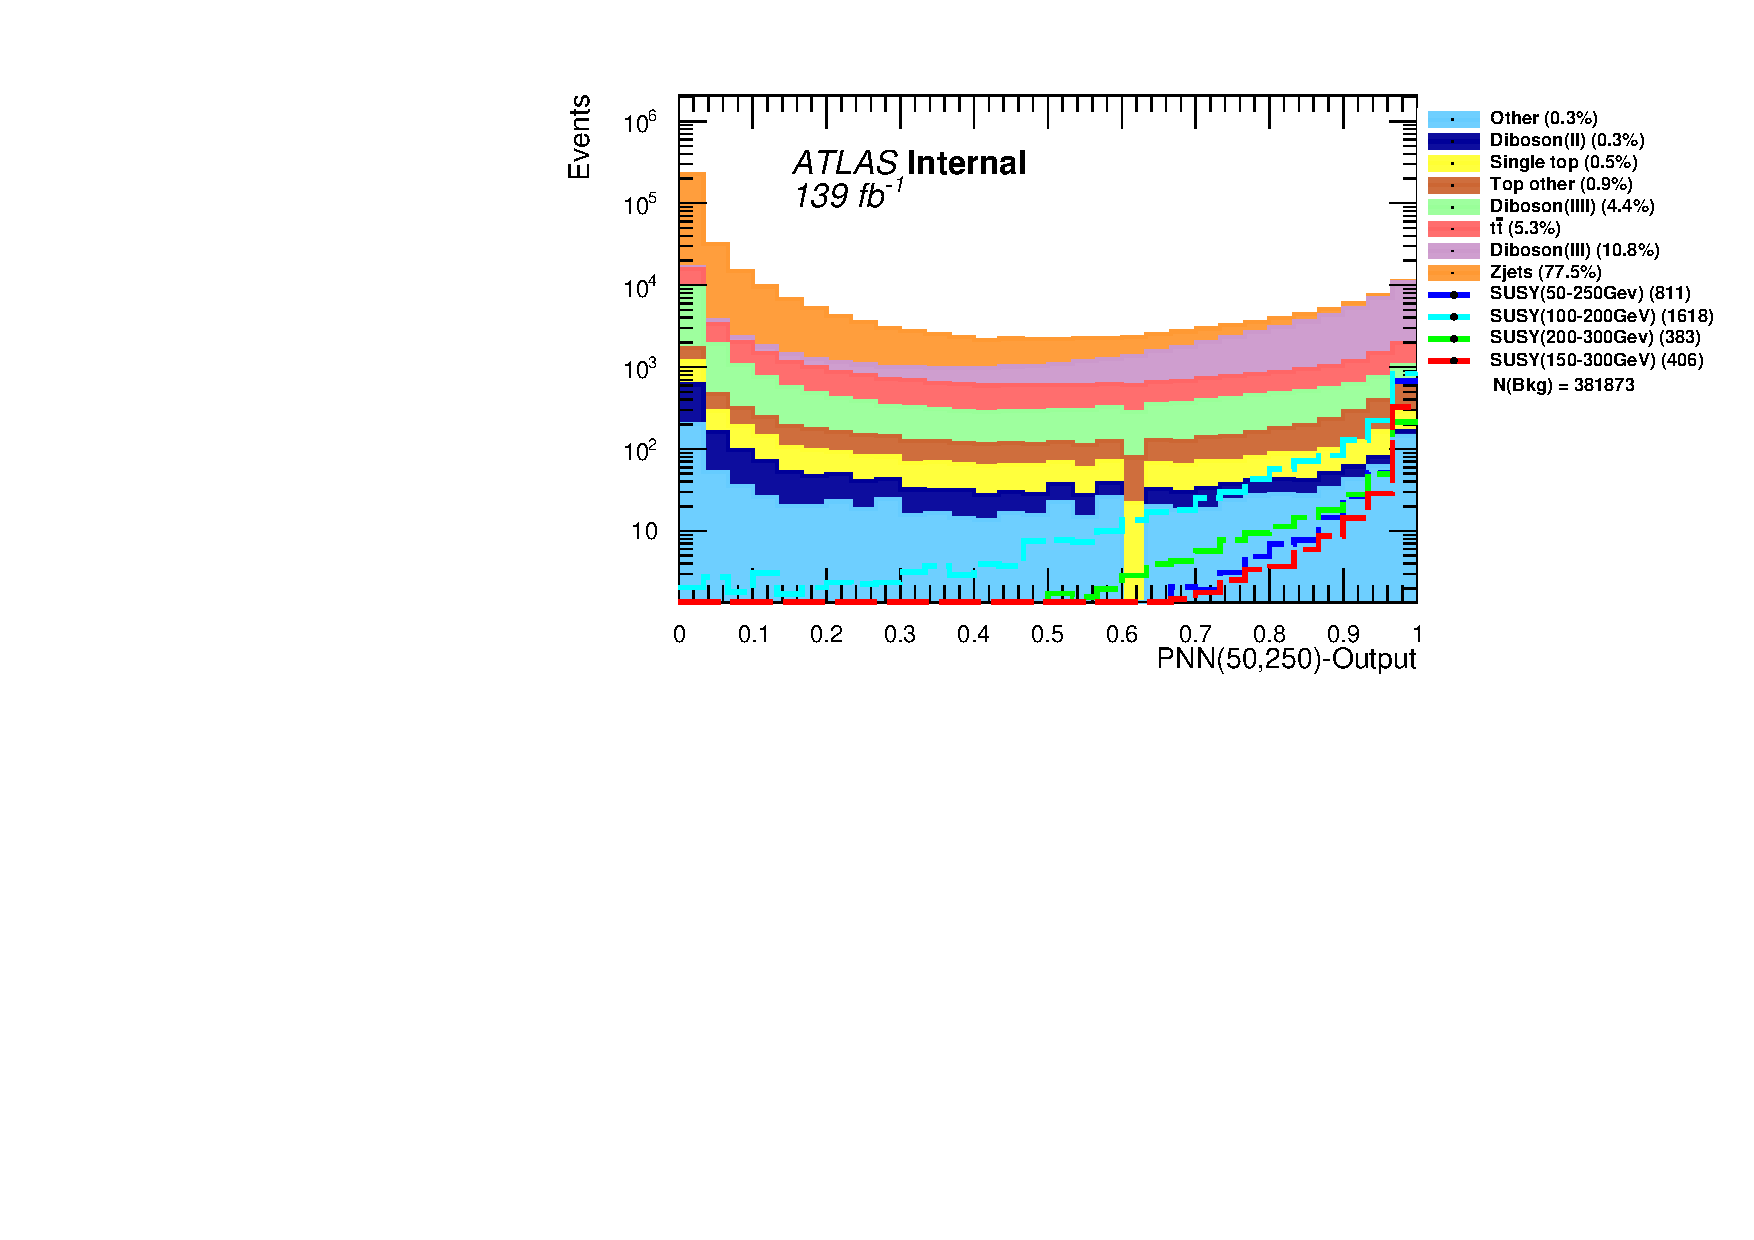
\includegraphics[width=\textwidth]{Figures/MLResults/NN/SUSY/MLDist/PNNDistTest/PNN50250Dist.pdf}
        \caption{}
        \label{fig:PNN50250Dist}
    \end{subfigure}
    \hfill
    \begin{subfigure}{.5\textwidth}
        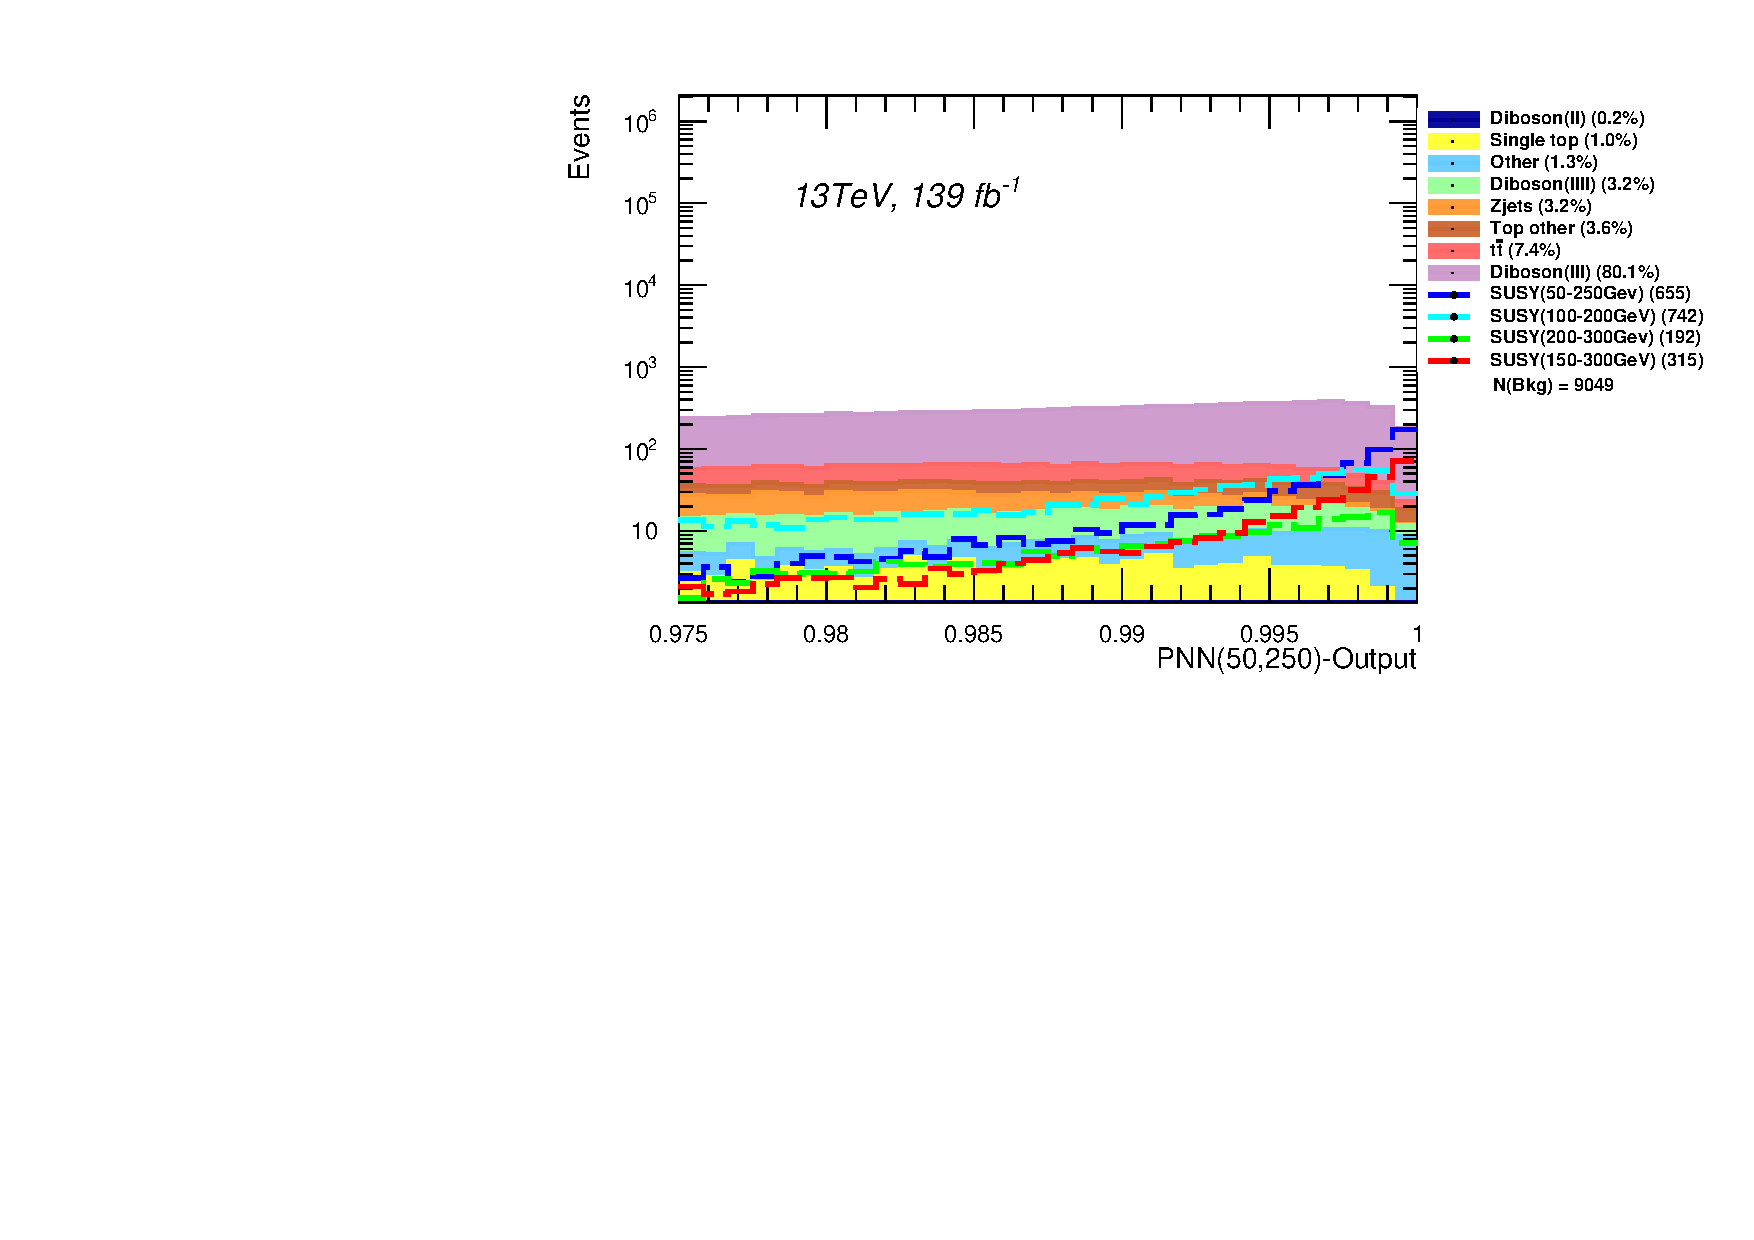
\includegraphics[width=\textwidth]{Figures/MLResults/NN/SUSY/MLDist/PNNDistTest/PNN50250Dist_C7.pdf}
        \caption{}
        \label{fig:PNN50250Dist_95}
    \end{subfigure}
    }
    \caption{The output distribution from a trained \ac{PNN} model for the background and signals with 4 different mass combinations:
    ($\tilde{\chi}_1=50$, $\tilde{\chi}_2=250$GeV), ($\tilde{\chi}_1=100$, $\tilde{\chi}_2=200$GeV), 
    ($\tilde{\chi}_1=200$, $\tilde{\chi}_2=300$GeV) and ($\tilde{\chi}_1=150$, $\tilde{\chi}_2=250$GeV), and where all the data were given the 
    parameter features of ($\tilde{\chi}_1=50$, $\tilde{\chi}_2=250$GeV). The figure includes the full output range (\ref{fig:PNN50250Dist}) 
    and the output ranging from 0.975-1.00 (\ref{fig:PNN50250Dist_95}).}
    \label{fig:PNN50250}
\end{figure}
\begin{figure}
    \makebox[0.95\linewidth][c]{%
    \centering
    \begin{subfigure}{.5\textwidth}
        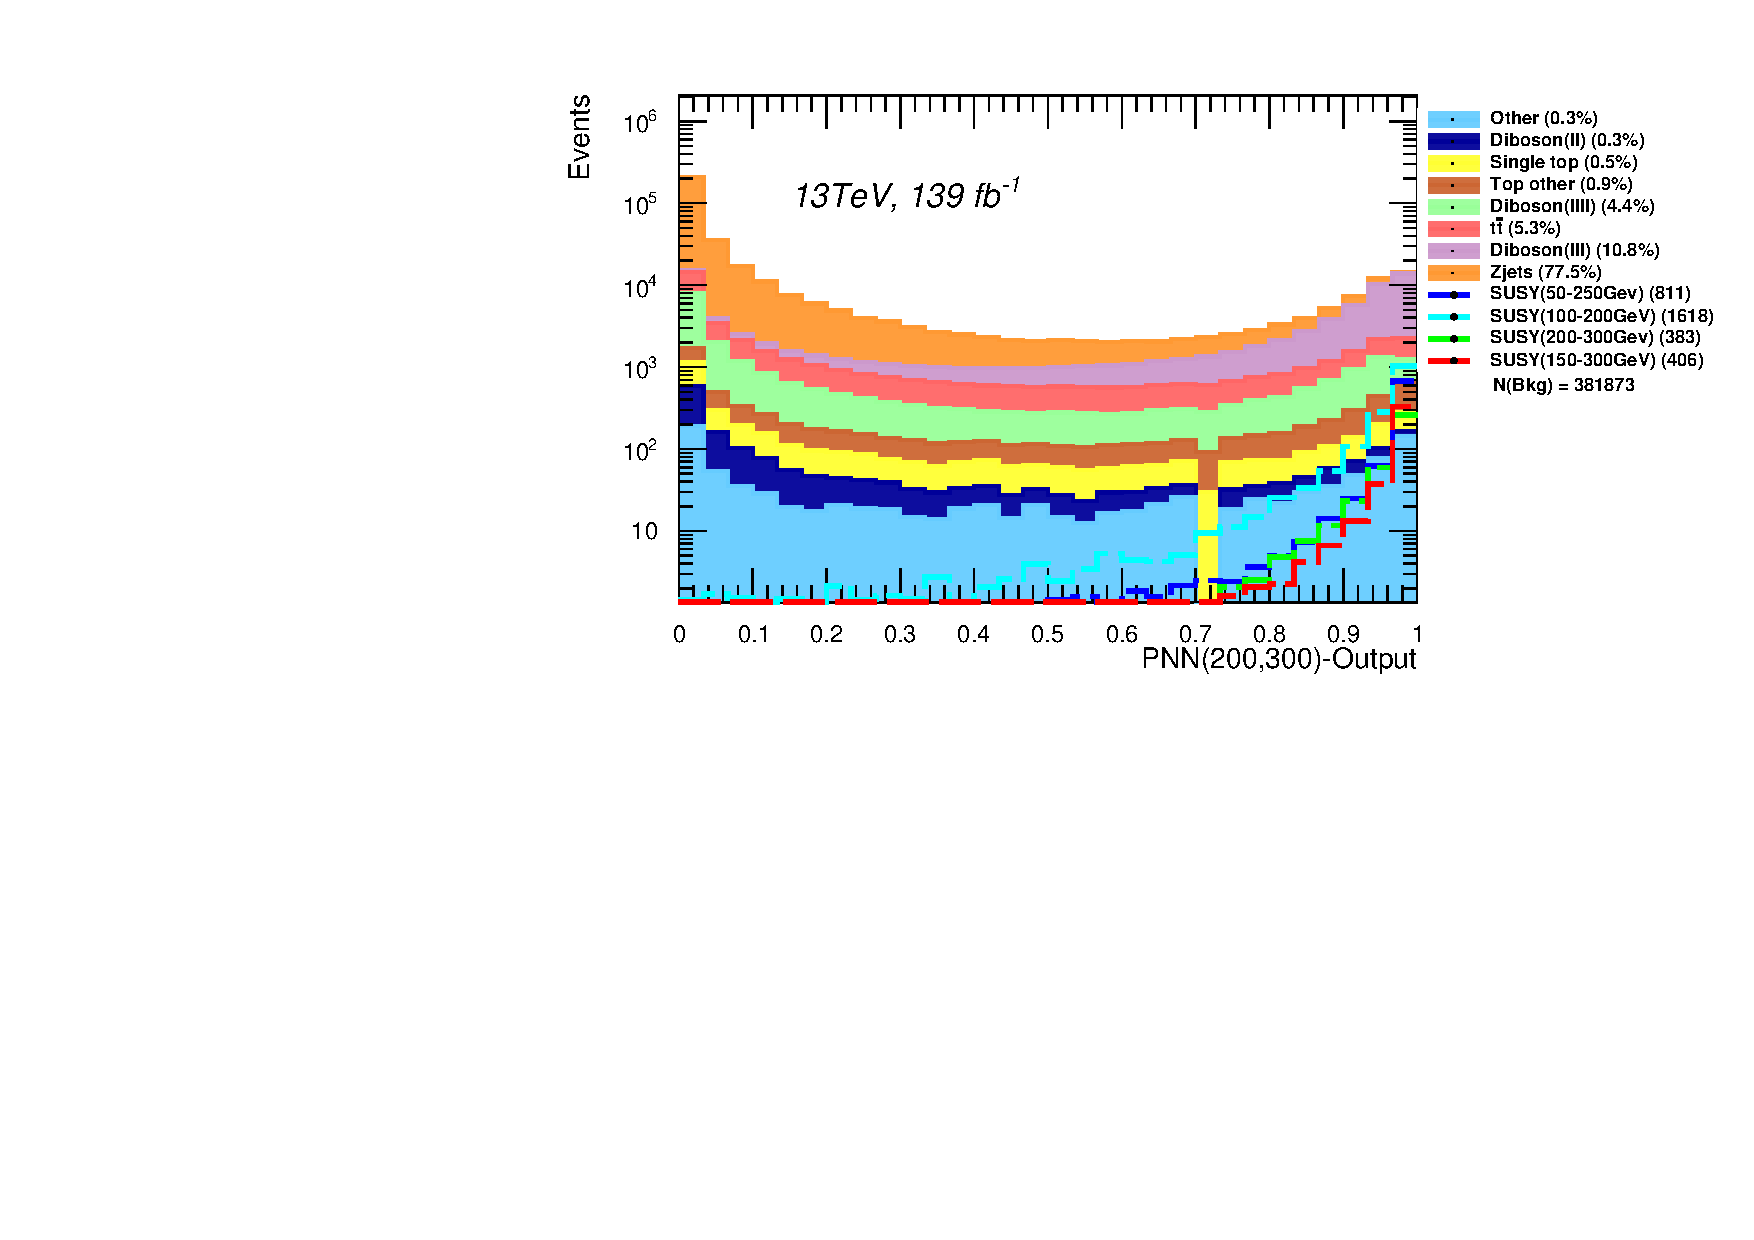
\includegraphics[width=\textwidth]{Figures/MLResults/NN/SUSY/MLDist/PNNDistTest/PNN200300Dist.pdf}
        \caption{}
        \label{fig:PNN200300Dist}
    \end{subfigure}
    \hfill
    \begin{subfigure}{.5\textwidth}
        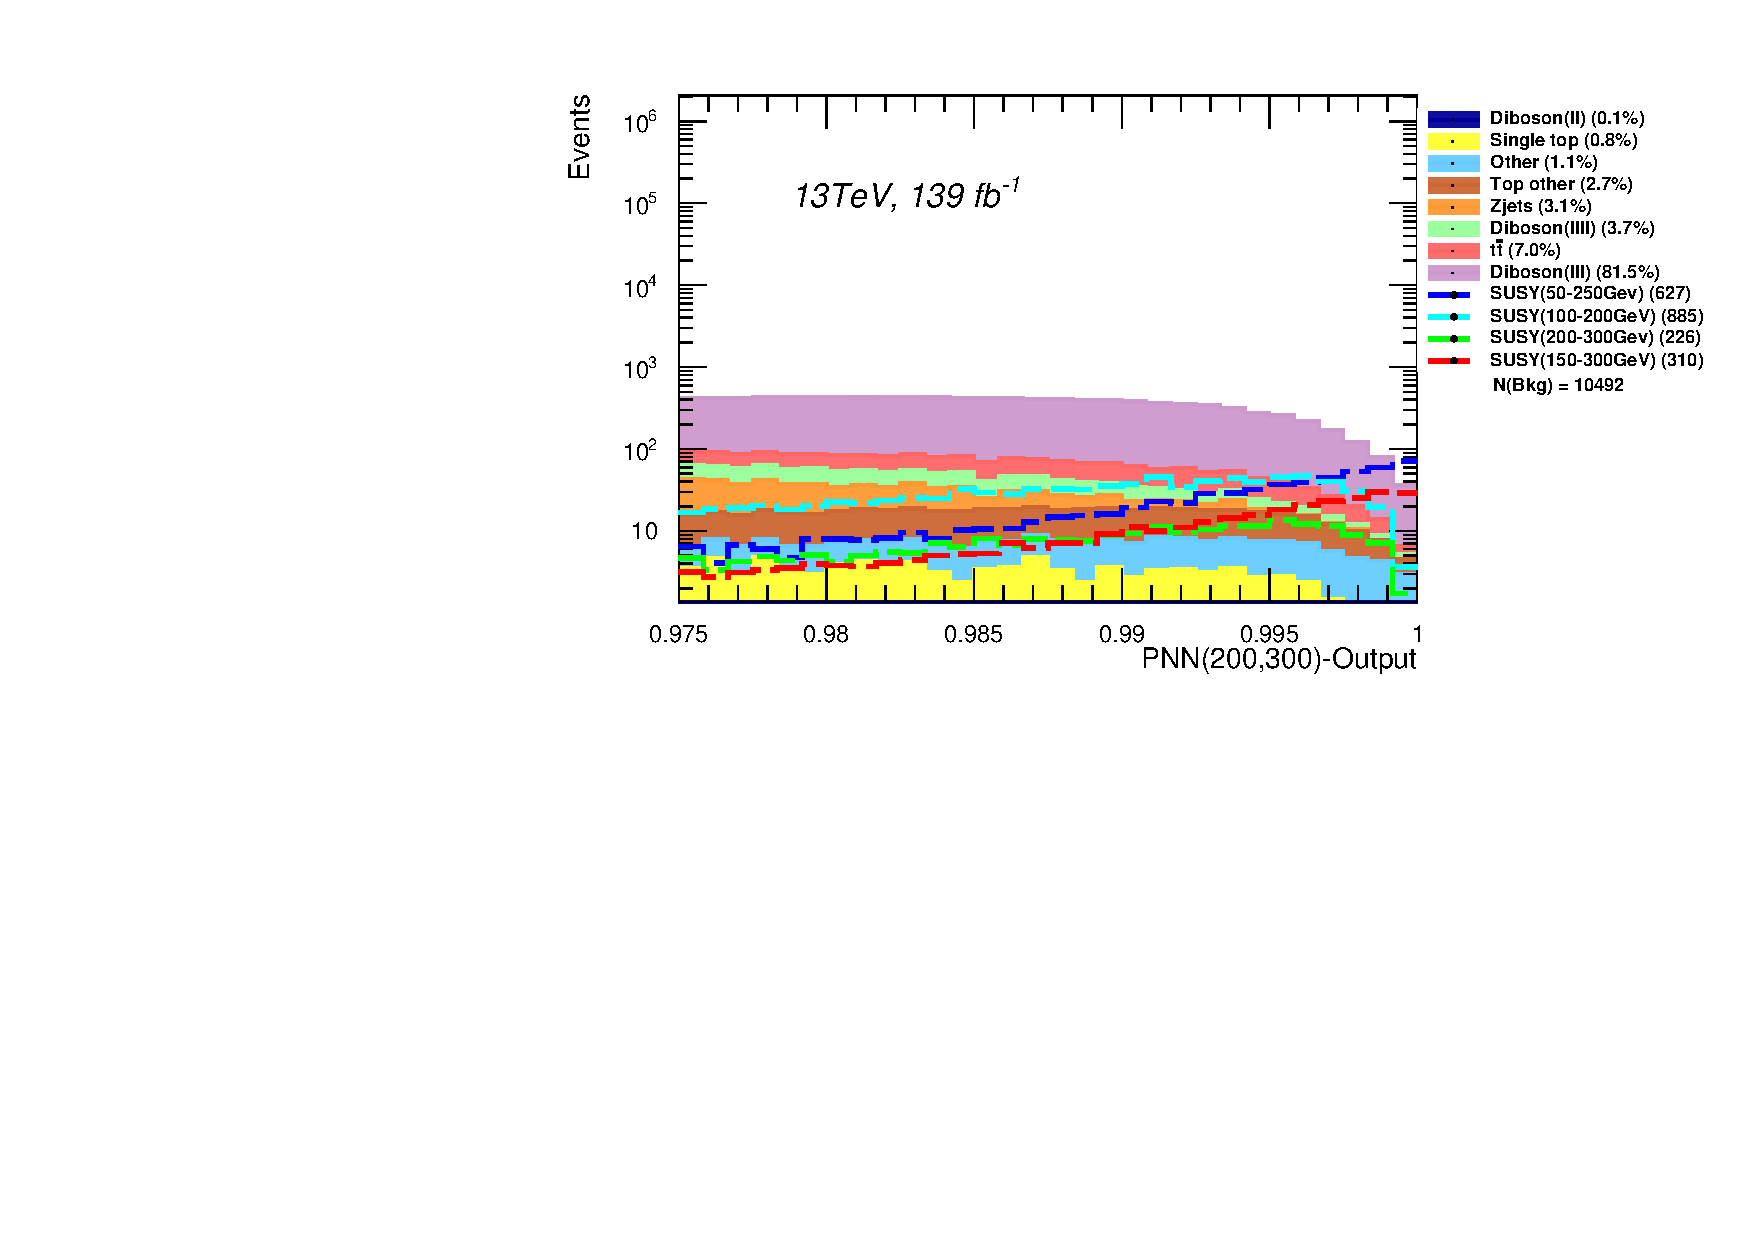
\includegraphics[width=\textwidth]{Figures/MLResults/NN/SUSY/MLDist/PNNDistTest/PNN200300Dist_C7.pdf}
        \caption{}
        \label{fig:PNN200300Dist_95}
    \end{subfigure}
    }
    \caption{The output distribution from a trained \ac{PNN} model for the background and signals with 4 different mass combinations:
    ($\tilde{\chi}_1=50$, $\tilde{\chi}_2=250$GeV), ($\tilde{\chi}_1=100$, $\tilde{\chi}_2=200$GeV), 
    ($\tilde{\chi}_1=200$, $\tilde{\chi}_2=300$GeV) and ($\tilde{\chi}_1=150$, $\tilde{\chi}_2=250$GeV), and where all the data were given the 
    parameter features of ($\tilde{\chi}_1=200$, $\tilde{\chi}_2=300$GeV). The figure includes the full output range (\ref{fig:PNN50250Dist}) 
    and the output ranging from 0.975-1.00 (\ref{fig:PNN50250Dist_95}).}
    \label{fig:PNN200300DistComp}
\end{figure}

\begin{table}
    \centering
    $
    \begin{array}{ccccc}
        \hline \text { \backslashbox{\textbf{Label}}{\textbf{Channel}} }  & \text {$(50,250)$}& \text {$(100,200)$} & \text {$(150,300)$} & \text {$(200,300)$} \\
        \hline\text {$(50,250)$}   & \text { $\bf{80.8}\%$ } & \text { $45.8\%$ } & \text { $\bf{77.5}\%$ } & \text { $50.1\%$ } \\
        \hline\text {$(200,300)$}   & \text { $77.3\%$ } & \text { $\bf{54.6}\%$ } & \text { $76.3\%$ } & \text { $\bf{59.0}\%$ } \\
        \hline
    \end{array}
    $
    \caption{A listing of the remaining procentage of each mass combination in the output range 0.95-1.00 using the 
    labels ($\tilde{\chi}_1=50$, $\tilde{\chi}_2=250$GeV) and ($\tilde{\chi}_1=200$, $\tilde{\chi}_2=300$GeV) respectively.}
\label{table:PNNSigComp}
\end{table}

\subsection{Sensitivity Result}
\begin{figure}
    \makebox[\linewidth][c]{%
    \centering
    \begin{subfigure}{.65\textwidth}
        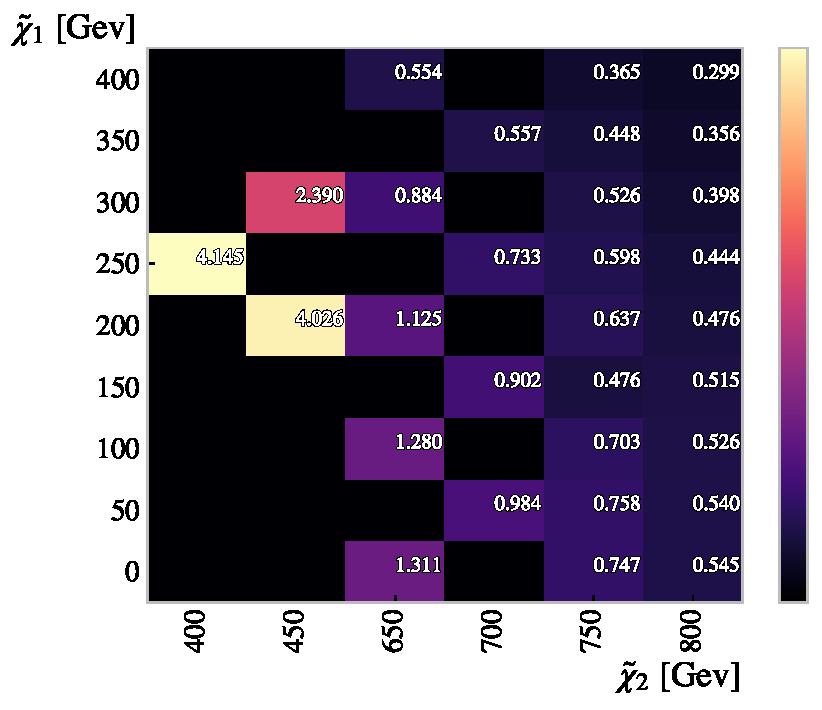
\includegraphics[width=\textwidth]{Figures/MLResults/NN/SUSY/Grid/PNNGridSig.pdf}
    \end{subfigure}
    }
    \caption{A grid displaying the achieved significance on the original signal set, using the signal region 
    created by the \ac{PNN} network.}
    \label{fig:PNNGridSig}
\end{figure}